\documentclass[12pt]{article}
\usepackage[margin=0.2in]{geometry}
\usepackage{amssymb}
\usepackage{amsmath}
\usepackage{url}
\usepackage{bm}
\usepackage{color}
\usepackage{graphicx}
\usepackage{cite}
\usepackage{caption}
\usepackage{subcaption}
\usepackage{hyperref}
\usepackage[section]{placeins} %keeps floats in their own section

\hypersetup{
    colorlinks,
    citecolor=blue,
    filecolor=blue,
    linkcolor=blue,
    urlcolor=blue
}

%\title{Plots for Alpha Formation in Mostly Neutron Matter}
%\author{Cody L. Petrie}

\begin{document}
%\maketitle
%\tableofcontents
%\newpage

Here are the latest calculations for the alpha formation in mostly neutron matter. I've done some calculations at different densities, not all of which are finished, but this is what I have in Figure~\ref{fig:alpha}.
\begin{figure}[h!]
   \centering
   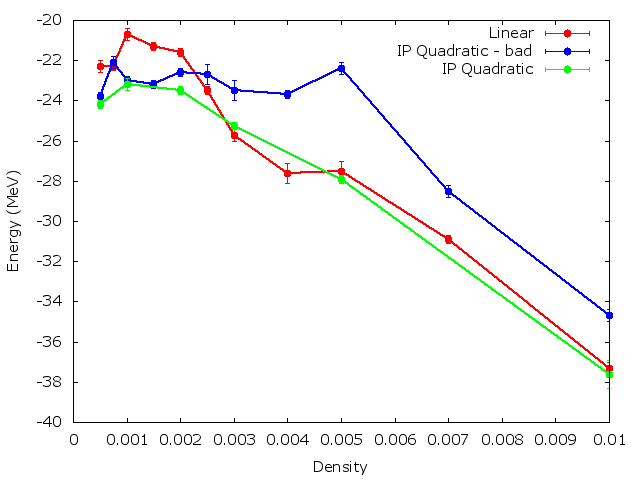
\includegraphics[width=0.60\textwidth]{../../alpha.png}
   \caption{Alpha energy calculated as $16\epsilon_{14n2p}-12\epsilon_{14n}$ where $\epsilon=E/A$.}
   \label{fig:alpha}
\end{figure}
It looks like the two correlations give about the same answer above $\rho=0.002$fm$^{-3}$, and the quadratic (IP) correlations give more binding below that density.

I also did calculations at the same densities with just 2 neutrons and 2 protons for comparison and as you can see in figure~\ref{fig:alpha_and_2n2p} however the two correlations give about the same answer, so the extra neutrons must be sensative to the extra correlations of the quadratic. Figure~\ref{fig:alpha_and_2n2p} also compares the 2n2p calculations to the cluster calculations in Figure~\ref{fig:alpha}.
\begin{figure}[h!]
   \centering
   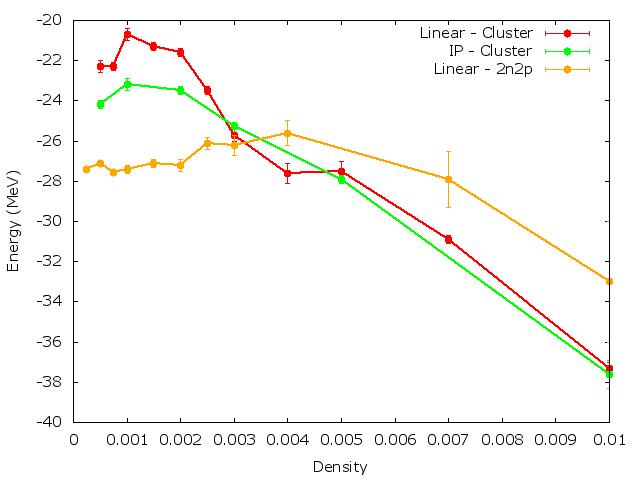
\includegraphics[width=0.60\textwidth]{../../alpha_and_2n2p.png}
   \caption{Energy of alpha particle calculated as a cluster in mostly neutron matter and 2 neutrons and 2 protons with both linear and IP correlations.}
   \label{fig:alpha_and_2n2p}
\end{figure}

I also plotted the separate pieces of the AV6' potential to see which pieces of the quadratic correlations mattered the most. Figure~\ref{fig:av6_alpha_linVSip} shows that the two pieces that differ the most are the OPE pieces, sigma-tau (vst in the plot) and tensor-tau (vtent in the plot). So this is good.
\begin{figure}[h!]
   \centering
   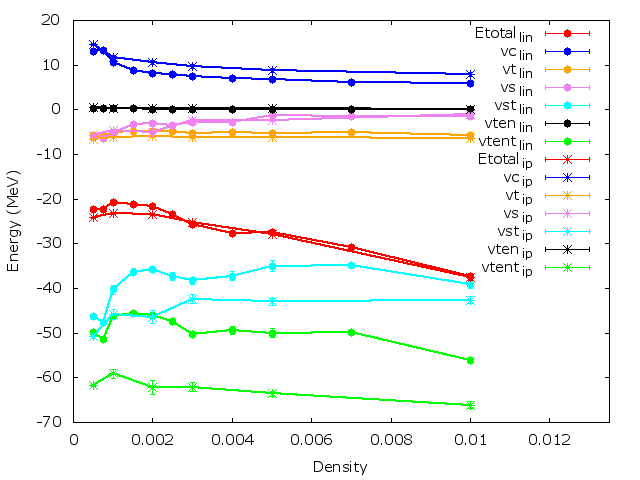
\includegraphics[width=0.60\textwidth]{../../av6_alpha_linVSip.png}
   \caption{Energy of alpha particle calculated as a cluster in mostly neutron matter and 2 neutrons and 2 protons with both linear and IP correlations.}
   \label{fig:av6_alpha_linVSip}
\end{figure}

I also compared the proton-proton correlations functions


\end{document}
